\chapter{Introduction}
\label{ch:intro}

This thesis aims to understand how an organism adapts its metabolism and cellular processes in response to external conditions, in the context of a biological rhythm.
Specifically, I use the yeast metabolic cycle (YMC) as a framework for biological rhythms.
My reasons are twofold: (a) biological rhythms are important for coordination of responses and are present across kingdoms, (b) there are unanswered questions about the mechanistic basis of the YMC and about reconciling evidence from two types of experimental studies.
%Therefore, I study YMC regulation in isolated cells in different nutrient conditions.

This thesis is divided into six chapters:
\begin{enumerate}
  \item Chapter~\ref{ch:intro} discusses the background behind the yeast metabolic cycle and using flavin autofluorescence as a way to monitor the yeast metabolic cycle.
  \item Chapter~\ref{ch:methods} discusses the methods: single-cell microfluidics of yeast strains, an automated image analysis pipeline, and time series analysis methods.
  \item Chapter~\ref{ch:biology} presents results from single-cell microfluidics and fluorescence microscopy to detect flavin-based metabolic cycles in yeast cells.
        I show that the metabolic cycle and cell division cycle are autonomous and synchronise in permissive conditions, while perturbations affect the relationship between these two biological oscillators.
  \item Chapter~\ref{ch:analysis} discusses the analysis of oscillatory time series.
        Given and the challenges of analysing noisy low-resolution time series, this deserves discussion in its own right.
        This chapter explores processes to visualise groups in the dataset, detecting rhythmicity, period estimation, and detecting synchrony.
  \item Chapter~\ref{ch:model} discusses using flux balance analysis to address whether proteome constraints explain sequential scheduling of biosynthesis in the yeast metabolic cycle.
  \item Finally, Chapter~\ref{ch:concl} presents a conclusion based on the previous three results chapters and suggests further avenues of study.
\end{enumerate}

\section{Biological rhythms}
\label{sec:intro-biological_rhythms}

\subsection{Biological basis of biological rhythms}
\label{subsec:intro-biological_rhythms-biological_basis}

Biological rhythms are repeating physiological or cellular processes.
Biological rhythms include the circadian rhythm, the cell division cycle, the glycolytic cycle, and the yeast metabolic cycle.
Genetic oscillators, biochemical oscillators, and metabolic oscillators, all linked to a cellular redox cycle, govern biological rhythms \parencite{mellorMolecularBasisMetabolic2016}.
Biological rhythms can occur at different time scales, from seconds, to ultradian cycles (more frequent than 24 hours), to circadian rhythms (24 hours).
Biological rhythms are important in temporally separating physiological processes.
This separation is instrumental in responding to external conditions, including nutrient conditions, growth requirements, or the day-night cycle.
%Thus, this means that biological rhythms can vary according to conditions.

To demonstrate the definition of biological rhythm, I discuss the cell division cycle, which is well-char\-ac\-terised, and the glycolytic cycle, which is less well-characterised.


\subsubsection{Cell division cycle}
\label{subsubsec:intro-cdc}

The cell division cycle is a series of cellular events that ensure that a parent cell divides into two progeny cells.
These events include cell growth and accumulation of biomass, replication of genetic material with proofreading, and dividing the cell into two compartments.
In eukaryotes, the latter event consists of karyokinesis (division of the nucleus) and cytokinesis (division of the cell).
In budding yeast (\textit{Saccharomyces cerevisiae}), the cell division cycle is divided into the G\textsubscript{1}, S, G\textsubscript{2}, and M phases (Fig.\ \ref{fig:intro-cdc-overview}).
In the gap phases (G\textsubscript{1} and G\textsubscript{2}), the cell primarily grows and accumulates biomass.
The cell replicates DNA in the S phase and in the M phase it conducts mitosis, in which chromosomes are segregated between the progeny cells.

\begin{figure}
  \centering
  \includegraphics[width=0.9\textwidth]{adlerYeastCellCycle2022_1}
  \caption[
    Overview of the cell division cycle
  ]{
    Overview of the cell division cycle in budding yeast.
    The cell division cycle consists of G\textsubscript{1}, S, G\textsubscript{2}, and M phases (black arrows).
    The cell expresses different cyclins (coloured curves), cell division cycle regulators, as it transitions through different phases of the cell division cycle.
    Adapted from \textcite{adlerYeastCellCycle2022}.}
  \label{fig:intro-cdc-overview}
\end{figure}

The cell division cycle is important in unicellular organisms such as budding yeast because it is the mechanism by which the organism reproduces.
Regulation of the cell division cycle is thus important
(a) because the cell must only divide when necessary,
(b) because the cell must have resources available for division before it divides,
(c) because the cell must ensure faithful replication of DNA to prevent deleterious mutations in progeny cells,
and (d) because the cell must ensure that its components are divided equally between the two progeny cells so that its progeny cells can function normally.
The cell division cycle in budding yeast has checkpoints between phases to ensure that biological events from the previous phases are completed before the cell proceeds to the next phase.
The most important checkpoint is START in late G\textsubscript{1} phase.
Upon START, the cell checks whether it has the resources needed to replicate, and if requirements are met, it irreversibly commits to cell division.
The cell division cycle in budding yeast is also governed by a series of gene regulatory networks that interact in a feedback loop, resulting in oscillatory expression of cyclin-CDK complexes that regulate cellular events in a temporal manner \parencite{adlerYeastCellCycle2022, orlandoGlobalControlCellcycle2008, murrayRecyclingCellCycle2004}.
Specifically, cyclins are proteins that sequentially accumulate and are destroyed as the cell transitions through phases of the cell division cycle.
In budding yeast, these cyclins bind to and activate the cyclin-dependent kinase (CDK) Cdc28, which is constitutively expressed.
The different cyclin-CDK combinations in each phase thus determines the events in the cell \parencite{adlerYeastCellCycle2022}:

\begin{enumerate}
  \item In early G\textsubscript{1}, Cln3-Cdc28 phosphorylates Whi5, leading to activation of genes that regulate budding and DNA replication.
  \item In late G\textsubscript{1}, Cln1-Cdc28 and Cln2-Cdc28 hyperphosphorylates Sic1, leading to activation of DNA replication which marks S phase.
  \item In late S phase, Clb1-Cdc28 and Clb2-Cdc28 phosphorylates Ndd1, leading to a feedback loop that activates entry into mitosis.
  \item To exit mitosis, the cell activates a system to target Clb1 and Clb2 for degradation.
\end{enumerate}

To coordinate cell division and metabolism with nutrient availability, budding yeast also has a system of cross-talk between nutrient signalling, growth, and the cell division cycle \parencite{ewaldHowYeastCoordinates2018}.
The cell integrates information from nutrient-sensing systems at START\@.
In response to carbon deprivation, Cip1 delays START, while Msa1/2 responds to nutrient depletion and blocks START\@.
In addition, Rim15 integrates information from the TOR and PKA pathways, which respond to nutrient depletion and other stresses, and induces cell division cycle arrest.
Rim15 also responds to nutrient-poor conditions like non-fermentable carbon sources by inducing an earlier entry into START\@.

Furthermore, there is also evidence that sudden starvation at other phases affects cell division cycle progression, for example, through the S-phase inhibitor Sic1.
The cell also coordinates internal nutrient stores with the cell division cycle.
During S/G\textsubscript{2}/M, Cdc28 activates the trehalase Nth1 so that the storage carbohydrate trehalose can be liquidised to provide glucose for glycolysis \parencite{ewaldYeastCyclinDependentKinase2016}.
Additionally, during G\textsubscript{1}/S, Cdc28 activates the lipase Tgl4 to break down storage lipids \parencite{kuratCdk1Cdc28DependentActivation2009}.
There is also evidence for an additional cyclin-dependent kinase, Pho85 \parencite{huangPho85MultifunctionalCyclindependent2007}, which inhibits the expression of genes involved in the phosphate starvation response in high levels of environmental phosphate \parencite{oneillRegulationPHO4Nuclear1996}, and also has roles in inhibiting glycogen synthase \parencite{wilsonSubstrateTargetingYeast1999}.


\subsubsection{Glycolytic cycle}
\label{subsubsec:intro-glycolytic}

The glycolytic oscillation is a biochemical oscillator in budding yeast, characterised by damped  oscillations in the levels of glycolytic intermediates at a period of 40--50 seconds  \parencite{ghoshOscillationsGlycolyticIntermediates1964}.
These oscillations have been observed as a response to high-glucose conditions and in anaerobic conditions.
Later studies show that levels of NADH \parencite{lloydSaccharomycesCerevisiaeOscillatory2019, olsenOscillationsYeastGlycolysis2021}, pH, and mitochondrial membrane potential \parencite{doddLiveCellImaging2017} also oscillate at the same frequency (Fig.\ \ref{fig:intro-glycolytic-overview}).

\begin{figure}
  \centering
  \includegraphics[width=0.7\textwidth]{doddLiveCellImaging2017_3a_adapted}
  \caption[
    Glycolytic cycles
  ]{
    Glycolytic cycles are characterised by oscillations in NADH (orange) and pH (blue) at a period of approximately 40--50 s, and are usually highly damped.
    Adapted from \textcite{doddLiveCellImaging2017}.}
  \label{fig:intro-glycolytic-overview}
\end{figure}

Many hypotheses have been proposed to explain the existence of glycolytic oscillations, but there is no consensus \parencite{lloydSaccharomycesCerevisiaeOscillatory2019}, though \textcite{thokeConstantLowentropyProcess2018} proposed that these oscillations are the result of cells attempting to maintain a constant low-entropy state while remaining metabolically active.
Evidence shows that glycolytic oscillations are regulated through solely biochemical means.
Specifically, a high ADP/ATP ratio and the presence of fructose-1,6-bisphosphate activate the activity of phosphofructokinase, which then controls the flux through glycolysis, forming a negative feedback loop that causes oscillations \parencite{ghoshOscillationsGlycolyticIntermediates1964, higginsChemicalMechanismOscillation1964}.
Such a biochemical mechanism would explain how oscillations are sustained at a short timescale.

\subsection{Mathematical basis of biological rhythms}
\label{subsec:intro-biological_rhythms-theoretical_basis}

% Single oscillations
% Useful here: cell division cycle modelling literature, e.g. Novak/Tyson,
% Adler et al. (2022) -- comprehensive review of cell division cycle models
% Goldbeter (2022) -- models of several examples
The mathematical modelling of biological rhythms originated in included simple systems of ordinary differential equations to describe negative feedback control circuits \parencite{goodwinOscillatoryBehaviorEnzymatic1965, griffithMathematicsCellularControl1968}.
Experimental observations have then informed the development of models with finer detail.
Furthermore, subsequent studies have modelled and synthesised artificial genetic circuits \parencite{elowitzSyntheticOscillatoryNetwork2000}.

The well-characterised cell division cycle has inspired models with a variety of approaches.
Early models are based on a negative feedback loop of key components as identified by experimental studies.
For example, \textcite{goldbeterMinimalCascadeModel1991} assumed a minimal model of one cyclin, one kinase, and one protease to construct a negative feedback loop with a delay, giving rise to stable oscillations.
Such a strategy forms the basis of later models that incorporate more detail, including additional control points of the cell division cycle \parencite{chenIntegrativeAnalysisCell2004}, responses to perturbations such as osmotic stress \parencite{adroverTimeDependentQuantitativeMulticomponent2011}, and relationship with other oscillators like the circadian rhythm \parencite{gerardEntrainmentMammalianCell2012, charvinForcedPeriodicExpression2009, droinLowdimensionalDynamicsTwo2019}.
More recent, comprehensive models include \textcite{adlerYeastCellCycle2022} which is based on a system of ordinary differential equations adapted for the modelling to pheromone and osmotic shock responses, and \textcite{novakMitoticKinaseOscillation2022}, which models the cell division cycle as a series of switches between two stable steady states whose behaviour is regulated by the CDK oscillator.

Models of glycolytic oscillations have less precision because the oscillation is less well-characterised.
Most models focus on few intermediates of glycolysis that would explain the observed oscillations.
\textcite{ghoshOscillationsGlycolyticIntermediates1964} proposed a simple biochemical mechanism governed by the action of phosphofructokinase, dependent on the concentration of fructose-1,6-bisphosphate.
\textcite{higginsChemicalMechanismOscillation1964} then tested this mechanism, by describing differential equations that model six chemical reactions.
Later, \textcite{termoniaOscillationsControlFeatures1981} incorporated pyruvate kinase kinetics and levels of AMP, ADP, and ATP as part of their kinetic model based on Michaelis-Menten kinetics.
Other studies focus on non-linear dynamics.
\textcite{goldbeterDissipativeStructuresAllosteric1972} models the product-activated phosphofructokinase reaction, taking into account the allosteric nature of the enzyme.
This model contains a single positive feedback loop as a instability-generating mechanism in a bistability model that explains oscillations.
In \textcite{moranOnsetBirhythmicityRegulated1984}, the model was modified to incorporate a reaction of product recycling into substrate to explain birhythmicity, namely, the potential for oscillations of different amplitudes.
Another development of the model includes a three-variable model that represents two coupled reactions each under a positive feedback loop, explaining more complex oscillatory phenomena that could arise from pulsing of substrates \parencite{decrolyBirhythmicityChaosOther1982}.
In contrast to work that models the cell division cycle, gene expression dynamics and the effects of perturbations have not been incorporated in the modelling of the glycolytic cycle.

% Forced oscillators, coupled oscillators
% Useful here: \textcite{tysonTimekeepingDecisionmakingLiving} and related reviews
As biological rhythms are often coupled with each other, forced and coupled oscillators have been modelled.
If an oscillator is forced, it has a natural oscillation frequency, but is forced from it due to an external force applied at a regular interval.
An example is the circadian clock, which is entrained to the light-dark cycle \parencite{goldbeterMultisynchronizationOtherPatterns}.
Yeast glycolytic oscillations can also be entrained via a periodic input of substrate.

Forced oscillators are closely linked to coupled oscillators, in which two oscillators are coupled to each other by certain activation or deactivation events.
Two coupled oscillators tend to oscillate at a compromise frequency if the natural frequencies of each are close enough to each other.
Otherwise, complex oscillations can occur: the oscillators lock to a rational ratio of frequencies --- i.e.\ one oscillator goes through $p$ periods while the other goes through $q$ periods.
In this case, the exact ratio depends on the ratio of the natural frequencies.
Furthermore, in certain cases, chaos can occur.
There is a mathematical basis in Arnold tongues \parencite{heltbergTaleTwoRhythms2021}.
Experimental observations support this.
For example, \textcite{charvinForcedPeriodicExpression2009} showed that externally forcing cell division cycles via glucose pulsing leads to phase-locking of the cell division cycle oscillator only within a range of extrinsic periods.


\section{Yeast metabolic cycle}
\label{sec:intro-ymc}

\subsection{Definition and description of the yeast metabolic cycle}
\label{subsec:intro-ymc-definition}
% Worth re-reading: Mellor 2016, Lloyd 2019

The yeast metabolic cycle is an ultradian biological rhythm which has been described to entail oscillations in oxygen consumption, metabolite concentrations, transcript levels, and cellular events, at the population level.
This yeast metabolic cycle is linked to the cell division cycle, but operates autonomously.

The yeast metabolic cycle is classed as a type of biological rhythm because it has the properties that define a biological rhythm.
Namely, it has gene-expression oscillators as evidenced by transcript cycling in its phases,
it has biochemical oscillators as evidenced by changes in dissolved oxygen in the chemostat,
and it has metabolite oscillations as evidenced by changes in the levels of compounds that undergo redox reactions like NADH/NADPH and flavins.

\subsubsection{Phases of the yeast metabolic cycle}
\label{subsubsec:intro-ymc-definition-phases}
% INTEGRATE THIS STRUCTURE IN EACH PARAGRAPH THAT DISCUSSES EACH PHASE
% 1. Overarching theme of phase
% 2. Cellular events (cell division cycle, mitochondria)
% 3. Metabolic events (metabolite concentrations, redox)
% 4. Transcript/genetic events.
% Or any that make sense, e.g. 3 main events and all the evidence from different
% parts of biochemistry.
% Structure should then link well with the definition of biological rhythms in
% a previous subsection.
% ---------------------------------------------------------------------

Based on chemostat studies,
the YMC can be divided into two major phases: an oxidative, high-oxygen consumption (OX/HOC) phase and a reductive, low-oxygen consumption (RED/LOC) phase (Fig.\ \ref{fig:intro-ymc-overview}).

\begin{figure}
  \centering
  \includegraphics[width=1.0\textwidth]{mellorMolecularBasisMetabolic2016_3c_adapted}
  \caption[
    Phases of the yeast metabolic cycle
  ]{
    Phases of the yeast metabolic cycle,
    with (left) high- (HOC) and low-oxygen consumption (LOC) phases defined by changes in dissolved oxygen concentration (dO\textsubscript{2}) over time in the chemostat
    and (right) oxidative (OX), reductive-building (RB) and reductive-charging (RC) phases defined by cycling of transcripts.
    Adapted from \textcite{mellorMolecularBasisMetabolic2016}.}
  \label{fig:intro-ymc-overview}
\end{figure}

% Though Lloyd/Murray camp also describe these 3 phases
Many authors \parencite{slavovMetabolicCyclingCell2011, murrayRedoxRegulationRespiring2011, caustonMetabolicRhythmsFramework2018} use oxygen consumption rates, evidenced by the change of dissolved oxygen concentrations over time, as a basis to refer to the YMC as a two-phase cycle (Fig.\ \ref{fig:intro-ymc-tu-oxygen}).
In contrast, some authors \parencite{machneYinYangYeast2012} base their two-phase model on the clustering of transcript level patterns.
\textcite{krishnaMinimalPushPull2018} interpret the oxidative phase as a growth state, while the reductive phase is a quiescent state.

\begin{figure}
  \centering
  \includegraphics[width=0.8\textwidth]{tuLogicYeastMetabolic2005_1}
  \caption[
    The yeast metabolic cycle has been described as spontaneous respiratory cycles
  ]{
    The yeast metabolic cycle has been described as spontaneous respiratory cycles of 4--5 hours, as evidenced by regular oscillations of dissolved oxygen in the chemostat, after a starvation period.
    Adapted from \textcite{tuLogicYeastMetabolic2005}.}
  \label{fig:intro-ymc-tu-oxygen}
\end{figure}

In contrast to the two-phase model, some authors identify a three-phase model with a reductive-building (RB) phase and a reductive-charging (RC) phase within the reductive phase.
This three-phase model is primarily based on cellular events, including clustering of transcript trajectories \parencite{tuLogicYeastMetabolic2005} (Fig.\ \ref{fig:intro-ymc-tu-transcripts}) and of metabolite concentration trajectories \parencite{tuCyclicChangesMetabolic2007}.

\begin{figure}
  \centering
  \includegraphics[width=1.0\textwidth]{tuLogicYeastMetabolic2005_3d_adapted}
  \caption[
    The yeast metabolic cycle is characterised by transcript cycling
  ]{
    The yeast metabolic cycle is characterised by transcript cycling.
    Such transcripts are divided into three clusters based on their patterns and phase relationship.
    The peaking of these transcripts correspond to the three (OX, RB, RC) phases of the yeast metabolic cycle.
    Adapted from \textcite{tuLogicYeastMetabolic2005}.}
  \label{fig:intro-ymc-tu-transcripts}
\end{figure}

Single-cell studies \parencite{papagiannakisAutonomousMetabolicOscillations2017, baumgartnerFlavinbasedMetabolicCycles2018} do not discuss phases as the single-cell microfluidic set-up does not allow live monitoring of transcription, and oxygen consumption rate can only be measured from chemostat cultures.
Such studies define the metabolic cycle as autonomous oscillations in metabolite levels in individual cells over time (Fig.\ \ref{fig:intro-ymc-overview-ss}).
In later chapters, I adhere to this single-cell definition because I perform a single-cell study of the yeast metabolic cycle.
% ---- I don't think any publication explicitly says this -- it's mostly just Kevin IIRC.  I suggest phrasing it differently, below
%However, others [INSERT CHAIN OF PUBLICATIONS HERE] debate the existence of the reductive-charging phase and argue that this phase is an artefact of cellular adaptation to glucose limitation or feast-and-famine conditions.
The two- or three-phase response may result from cellular adaptation to glucose limitation in chemostat cultures, and it is unknown whether these dynamics hold true in glucose-rich conditions, which cannot be created in a chemostat \parencite{slavovCouplingGrowthRate2011}.

\begin{figure}
  \centering
  \includegraphics[width=1.0\textwidth]{zylstraMetabolicDynamicsCell2022_1}
  \caption[
    The yeast metabolic cycle seen as coordinated cycling of metabolites in the cell
  ]{
    The yeast metabolic cycle seen as coordinated cycling of metabolites in the cell, generated autonomously of the cell division cycle, but are linked in permissive conditions.
    Adapted from \textcite{zylstraMetabolicDynamicsCell2022}.}
  \label{fig:intro-ymc-overview-ss}
\end{figure}

Cellular processes occur with the phases of the metabolic cycle (Fig.\ \ref{fig:intro-ymc-overview-oneill}).
In the oxidative phase, cells consume oxygen at a high rate as respiration, fermentation, and
% Potentially may be the reason auxotrophs (hypothetically) don't have YMCs --
% but I showed that they do
energy-demanding processes
like biosynthesis and gene expression occur.
Biosynthesis and associated gene expression are confirmed by increased transcripts from genes encoding components of the translation machinery and amino acid biosynthesis \parencite{tuLogicYeastMetabolic2005}.
`Redox state' metabolites, including NADH, NADPH, glutathione \parencite{lloydUltradianMetronomeTimekeeper2005}, and flavins (FMN and FAD)
\parencite{murrayRedoxRegulationRespiring2011} become most oxidised in this phase.
As cells transition from the oxidative to the reductive phase, 70\% of metabolite concentrations peak, when NAD(P)H autofluorescence peaks, and the DNA synthesis rate is at its maximum \parencite{lloydTemporalArchitectureEukaryotic2006}.

\begin{figure}
  \centering
  \includegraphics[width=0.9\textwidth]{oneillEukaryoticCellBiology2020_3a_adapted}
  \caption[
    The yeast metabolic cycle seen as sequential scheduling of cellular processes into phases
  ]{
    The yeast metabolic cycle seen as sequential scheduling of cellular processes into phases.
    Here, in the low-oxygen consumption (LOC) phase, the cell accumulates carbohydrates, amino acids, and solutes.
    In contrast, in the high-oxygen consumption (HOC) phase, the reverse is true:
    the cell uses its accumulated resources for biosynthesis and translation.
    Once reserves are exhausted, the cell resumes its LOC phase.
    Adapted from \textcite{oneillEukaryoticCellBiology2020}.}
  \label{fig:intro-ymc-overview-oneill}
\end{figure}

In the reductive phase, cells consume oxygen at a low rate.
During the reductive-building phase, activities linked to mitochondrial growth occur.
In the early reductive-building phase, ethanol and acetate concentrations in the medium peak, marking a transition from oxidative respiration to glycolytic metabolism \parencite{tuCyclicChangesMetabolic2007}.
There is evidence to suggest that activities linked to cell proliferation --- such as initiation of the cell division cycle, DNA replication, and spindle pole activity --- are gated to the reductive-building phase for both the short-period and long-period YMC\@.
Such evidence includes budding activity and the pattern of the expression of \textit{YOX1}, which encodes a cell division cycle repressor \parencite{tuLogicYeastMetabolic2005}.

% There are many strings to pull on this phase.
Finally, during the reductive-charging phase,
non-respiratory metabolism and degradation processes occur to prepare the cell for the oxidative phase.
This non-respiratory metabolism includes glycolysis, ethanol and fatty acid metabolism, and nitrogen metabolism.
With these metabolic modes, under the regulation of the transcription factors Msn2p and Msn4p \parencite{kuangMsn2RegulateExpression2017}, acetyl CoA accumulates so ATP can be produced in the oxidative phase \parencite{tuLogicYeastMetabolic2005}.
After acetyl CoA levels reach a threshold, it promotes histone acetylation and thus induces the oxidative phase.
These metabolic pathways also optimise production of NADPH --- based on the induction of \textit{GND2} --- to buffer against oxidative stress in the oxidative phase.
Genes associated with protein degradation, ubiquitinylation, peroxisomes, vacuoles, and the proteosome also peak in the reductive-charging phase.

It has been hypothesised that gating activities linked to cell proliferation to the reductive-building phase
creates a temporal separation between oxidative biochemical processes and the cell division cycle.
This temporal separation may prevent reactive oxygen species generated by oxidative process from damaging DNA\@.
However, measuring DNA content and oxygen consumption in cells grown at different growth rates \parencite{slavovCouplingGrowthRate2011} showed that the S phase of the cell cycle may occur in the oxidative phase if the cells have a slow growth rate.
% Not sure if they changed the growth rate of the cells though -- probably quite difficult
% to do in microfluidics setting.
% Re-phrase it a little to make it more different from Papagiannakis et al.
This may be explained by the YMC gating the early and late cell cycle independently, as evidenced by periodic localisation of the anaphase-promoting complex and mitotic exit activator Cdc14 phosphatase in metaphase-arrested cells \parencite{luPeriodicCyclinCdkActivity2010} and, conversely, the persistence of NAD(P)H cycling upon arresting of the late cell cycle by depletion of Cdc14 \parencite{papagiannakisAutonomousMetabolicOscillations2017}, all observed in single cells.
% What would be the function of such flexible gating?  Seems like community
% has no meaningful consensus yet.  Probably allocation of metabolites.
This evidence indicates that the gating between the YMC and the cell cycle is flexible.
Although there is no consensus on the function of such flexible gating,
gating can aid the allocation of metabolites to different temporal phases of both cellular oscillators.
% Discuss allocation of metabolites later -- and this can be linked to the modelling chapter of thesis.

\subsubsection{History of evidence for the yeast metabolic cycle}
\label{subsubsec:intro-ymc-definition-history}


Aspects of the YMC have been observed over decades.
\textcite{nosohSYNCHRONIZATIONBUDDINGCYCLE1962} discovered that synchronised \textit{S. cerevisiae} cultures show oscillatory oxygen consumption.
\textcite{kasparvonmeyenburgEnergeticsBuddingCycle1969} showed that gas metabolism and energy generation increase upon budding, while \textcite{mochanRespiratoryOscillationsAdapting1973} described a high-amplitude respiratory oscillation following a substrate shift from glucose to ethanol.
\textcite{satroutdinovOscillatoryMetabolismSaccharomyces1992} were the first to describe the metabolic components of a 40-minute YMC for cells in continuous culture.
\textcite{tuLogicYeastMetabolic2005}
first incorporated transcript cycling in the description of the YMC and defined the YMC events
based on a chemostat-based investigation of growth of budding yeast on glucose-starved conditions.

The yeast metabolic cycle is longer and is more robust than a similar biological oscillator, the glycolytic oscillation.
The glycolytic oscillation has a period of approximately 40 seconds \parencite{olsenRegulationGlycolyticOscillations2009}.
In contrast, the yeast metabolic cycle has been described, using various definitions, to either exhibit a 40-minute short-phase cycle \parencite{lloydUltradianMetronomeTimekeeper2005, liRapidGenomescaleResponse2006, lloydRedoxRhythmicityClocks2007}, or a long-phase cycle, which is most commonly described to be 4--5 hours \parencite{tuLogicYeastMetabolic2005, tuCyclicChangesMetabolic2007}, but also ranges between 1.4 hours to 14 hours, depending on the chemostat dilution rate \parencite{beuseEffectDilutionRate1998}.
Glycolytic oscillations are highly damped, but yeast metabolic oscillations are robust, lasting for weeks \parencite{lloydRedoxRhythmicityClocks2007}.
Additionally, glycolytic oscillations have been observed in anaerobic conditions \parencite{lloydSaccharomycesCerevisiaeOscillatory2019}, but yeast metabolic cycles have been observed in aerobic conditions.
Moreover, glycolytic oscillations are characterised by fluctuations in NADH fluorescence and glycolytic intermediates.
However, yeast metabolic cycles consist of fluctuations in NADH fluorescence, flavin fluorescence, and ATP concentrations as well as biosynthetic intermediates in TCA cycle, amino acid, and nucleic acid metabolism \parencite{tuCyclicChangesMetabolic2007}.


\subsection{Yeast metabolic cycles under perturbations}
\label{subsec:intro-ymc-perturbations}
% - Nutrient perturbations
  % - Changing concentration or compositions of carbon sources.
  % - Changing concentration or compositions of nitrogen sources.
  % - Key deletion strains shed light on mechanism

Perturbations in growth conditions can affect the length of the metabolic cycle and its relationship with other cellular events.
The long-phase cycle may vary from 1.4 to 14 hours \parencite{caustonMetabolicRhythmsFramework2018}.
The main nutrient perturbations that have been studied are perturbations in carbon sources and in nitrogen sources.

\subsubsection{Perturbations in growth conditions}
\label{subsubsec:intro-ymc-perturbations-nutrient}


Perturbations in carbon sources are well-documented.
% change glucose concentration
Lower glucose concentrations prolong the metabolic cycle, as evidenced by both chemostat studies that assess the effect of changing the dilution rate \parencite{burnettiCellCycleStart2016, oneillEukaryoticCellBiology2020} and by single-cell studies that assess the effect of glucose concentrations in the limiting region \parencite{papagiannakisAutonomousMetabolicOscillations2017}.
% 20 g/L --> 0.5 g/L doesn't seem to significantly prolong it, but maybe
% a greater effect will be seen if we get to the region of glucose limitation
% Though I am aware that this is my experimental observations -- need to see if literature confirms.
For example, decreasing the dilution rate decreases the growth rate, and in turn increases the duration of the oxidative phase relative to the reductive phases \parencite{slavovCouplingGrowthRate2011}, thus prolonging the metabolic cycle.
This effect is pronounced in the region of glucose limitation.
Increasing the glucose concentration beyond a certain point does not produce an effect.
Additionally, several studies \parencite{slavovCouplingGrowthRate2011,oneillEukaryoticCellBiology2020} show that the duration of the low oxygen consumption phase increases while the duration of the high oxygen consumption phase holds constant if the metabolic cycle duration increases due to these reasons.

Such experimental observations could by explained by models such as \textcite{jonesCyberneticModelGrowth1999}, which suggest that as the dilution rate is decreased, metabolic oscillations acquire greater amplitudes and longer periods, but if it is low enough, metabolism becomes entirely oxidative, and metabolic oscillations disappear.
% ferm vs non-ferm
However, non-fermentable carbon sources like pyruvate give long-duration metabolic cycles in single cells, comparable to cells under limiting levels of glucose \parencite{papagiannakisAutonomousMetabolicOscillations2017}.

% bulk addition and depletion
In addition, bulk depletion or addition of a carbon source can reset the phase of the YMC\@.
%Chemostat studies show that an initial starvation phase is needed to generate long-lasting synchronous metabolic cycles \parencite{tuLogicYeastMetabolic2005}. %[OTHER CITATIONS PROBABLY USEFUL].
%On the other hand,
Adding a bulk carbon source such as acetate, ethanol, or acetaldehyde can reset the phase of the YMC \parencite{kuangMsn2RegulateExpression2017, krishnaMinimalPushPull2018} or eliminate it \parencite{jonesCyberneticModelGrowth1999}.

Perturbations in nitrogen sources are less well-studied.
% Maybe also because long OX stage as it's the stage for biomass building
\textcite{baumgartnerFlavinbasedMetabolicCycles2018}, based on single-cell observations, suggest that decreasing nitrogen concentration prolongs the YMC, as evidenced by longer flavin oscillations when cells are grown on lower concentrations of yeast nitrogen base (YNB) media or on urea, a non-preferred nitrogen source.

In addition, perturbations outside nutrient sources also affect the YMC.\@
For example, externally applied hydrogen peroxide, as a source of oxidative stress, shifts the YMC to the oxidative phase \parencite{amponsahPeroxiredoxinsCoupleMetabolism2021}.
% [MOVED FROM PREVIOUS SECTION]
The oscillation period is insensitive to temperatures from \SI{25}{\celsius} to \SI{35}{\celsius} and media pH values from
2.9 to 6.0 \parencite{lloydUltradianMetronomeTimekeeper2005} --- though the period of dissolved-oxygen oscillations decrease as pH decreases to below 2.9 and the oscillations disappear when conditions are too acidic \parencite{oneillEukaryoticCellBiology2020}.
Additionally, the dissolved-oxygen oscillations are robust to media potassium ion concentrations varying between 1 and 10 mM, but disappear when the potassium concentration falls below 1 mM \parencite{oneillEukaryoticCellBiology2020}.

%Finally, the phase difference between the YMC and cell cycle varies in different conditions \parencite{ewaldYeastCyclinDependentKinase2016}.

\subsubsection{Genetic perturbations}
\label{subsubsec:intro-ymc-perturbations-genetic}

Although the molecular basis of the yeast metabolic cycle is not well-characterised, gene deletions shed light on it.
% Mellor (2016) provide an awesome table.
Genes that control the cell division cycle and metabolism have been deleted in studies.

Several deletions have been shown to remove the metabolic oscillations in chemostats: \textit{zwf1$\Delta$} \parencite{tuCyclicChangesMetabolic2007}, \textit{gsy2$\Delta$}, and \textit{gph1$\Delta$} \parencite{oneillEukaryoticCellBiology2020} (Figs.\ \ref{fig:intro-ymc-zwf1},~\ref{fig:intro-ymc-gsy2-gph1}).

\begin{figure}
  \centering
  \begin{subfigure}[htpb]{0.9\textwidth}
   \centering
   \includegraphics[width=\textwidth]{tuCyclicChangesMetabolic2007_2c_adapted}
   \caption{
   }
   \label{fig:intro-ymc-zwf1}
  \end{subfigure}
  \begin{subfigure}[htpb]{0.4\textwidth}
   \centering
   \includegraphics[width=\textwidth]{oneillEukaryoticCellBiology2020_5a_adapted}
   \caption{
   }
   \label{fig:intro-ymc-gsy2-gph1}
  \end{subfigure}
  \begin{subfigure}[htpb]{0.4\textwidth}
   \centering
   \includegraphics[width=\textwidth]{caustonMetabolicCyclesYeast2015_2e_adapted}
   \caption{
   }
   \label{fig:intro-ymc-rim11}
  \end{subfigure}
  \begin{subfigure}[htpb]{0.4\textwidth}
   \centering
   \includegraphics[width=\textwidth]{caustonMetabolicCyclesYeast2015_1e_adapted}
   \caption{
   }
   \label{fig:intro-ymc-swe1}
  \end{subfigure}
  \begin{subfigure}[htpb]{0.4\textwidth}
   \centering
   \includegraphics[width=\textwidth]{caustonMetabolicCyclesYeast2015_4a_adapted}
   \caption{
   }
   \label{fig:intro-ymc-tsa1-tsa2}
  \end{subfigure}
  \caption[
    Effects of genetic perturbations on the yeast metabolic cycle
  ]{
    Effects of genetic perturbations on the yeast metabolic cycle, as evidenced by the dissolved oxygen cycles of deletion strains observed in the chemostat.
    %
    \textbf{(\ref{fig:intro-ymc-zwf1})}
    \textit{zwf1$\Delta$} shows no dissolved oxygen cycles.
    Adapted from \textcite{tuCyclicChangesMetabolic2007}.
    %
    \textbf{(\ref{fig:intro-ymc-gsy2-gph1})}
    \textit{gsy2$\Delta$} and \textit{gph1$\Delta$} show no dissolved oxygen cycles.
    Adapted from \textcite{oneillEukaryoticCellBiology2020}.
    %
    \textbf{(\ref{fig:intro-ymc-rim11})}
    \textit{rim11$\Delta$} shows shorter dissolved oxygen cycles.
    Adapted from \textcite{caustonMetabolicCyclesYeast2015}.
    %
    \textbf{(\ref{fig:intro-ymc-swe1})}
    \textit{swe1$\Delta$} shows shorter dissolved oxygen cycles and a modified coupling ratio between the metabolic and cell division cycle oscillators.
    Adapted from \textcite{caustonMetabolicCyclesYeast2015}.
    %
    \textbf{(\ref{fig:intro-ymc-tsa1-tsa2})}
    \textit{tsa1$\Delta$ tsa2$\Delta$} shows dissolved oxygen cycles of a different shape.
    Adapted from \textcite{caustonMetabolicCyclesYeast2015}.
  }
  \label{fig:intro-ymc-del}
\end{figure}

\textit{ZWF1} codes for glucose-6-phosphate dehydrogenase and is thus responsible for entry into the pentose phosphate pathway and subsequently a major source of NADPH generation.
Therefore, deleting this gene may impair control of cellular redox.
However, because of its role, this gene deletion impairs adapting to oxidative and pH stress and also causes methionine auxotrophy, so it may be difficult to draw conclusions from this deletion in particular.
Furthermore, Idp2p and Ald6p catalyse reactions that generate NADPH and have shown to compensate for the loss of \textit{ZWF1} when cells are grown on lactate plates or on liquid cultures with glucose as the carbon source \parencite{minardSourcesNADPHYeast2005}.
This observation therefore raises the question of just how important \textit{ZWF1} is to the yeast metabolic cycle, and to what extent is NADPH generation needed for control of cellular redox.

On the other hand, \textit{GSY2} has a role in glucose storage and \textit{GPH1} has a role in glycogen mobilisation.
The absence of dissolved oxygen cycles in the associated deletions thus suggests that cycling of carbohydrate stores may be needed for the function of the metabolic cycle.
However, metabolic oscillations have been observed in high-glucose conditions \parencite{papagiannakisAutonomousMetabolicOscillations2017, baumgartnerFlavinbasedMetabolicCycles2018} in which glycogen synthesis is repressed.
These observations therefore suggest that glycogen cycling may play a more minor role in defining the yeast metabolic cycle and another nutrient cycling phenomenon may be more responsible.

In addition, \textit{MSN2} and \textit{MSN4} have been shown to regulate acetyl CoA accumulation in the reductive-charging phase, as evidenced by the lack of YMCs in deletion strains \parencite{kuangMsn2RegulateExpression2017}.
This observation suggests that genes involved in signalling pathways also play an important role in the integrity of the metabolic cycle.

Additionally, other deletions have been shown to change the frequency or shape of dissolved oxygen cycles.
\textcite{caustonMetabolicCyclesYeast2015} provide several examples, of which I discuss \textit{rim11$\Delta$}, \textit{swe1$\Delta$}, and \textit{tsa1$\Delta$ tsa2$\Delta$}. % they actually had more, but these are the three that pop in my head right now

Rim11p is the yeast homolog of the GSK3$\beta$ serine/threonine kinase, which regulates metabolism and plays a role in setting the speed of the circadian clock.
The \textit{RIM11} deletion has been shown to give shortened periods of dissolved-oxygen metabolic cycles in the chemostat, thus pointing towards a common mechanism for both biological oscillators (Fig.\ \ref{fig:intro-ymc-rim11}).

Swe1p is a conserved cell division cycle regulator that functions at the G2/M checkpoint and has roles in coupling the cell division cycle with the circadian rhythm.
Deleting \textit{SWE1} also resulted in shortened periods of dissolved-oxygen metabolic cycles but with the same rate of DNA replication, suggesting a dysregulation in the coupling between the yeast metabolic cycle and the cell division cycle (Fig.\ \ref{fig:intro-ymc-swe1}).

Tsa1p and Tsa2p are paralogous cytoplasmic thioredoxin peroxidases that cooperate in the peroxiredoxin-thioredoxin system to eliminate reactive oxygen species and have been shown to be a marker for circadian rhythms.
A double deletion of the two genes still results in metabolic cycles, but with an additional burst in high oxygen consumption during what would otherwise be the reductive-charging phase, showing that the peroxiredoxin-thioredoxin system is instrumental in the integrity of the yeast metabolic cycle (Fig.\ \ref{fig:intro-ymc-tsa1-tsa2}).
In addition, \textcite{amponsahPeroxiredoxinsCoupleMetabolism2021} show the presence of cycling peroxiredoxin oxidation during the YMC using chemostat-based studies, with a corresponding cycling of hydrogen peroxide.
They also confirm that inactivating peroxiredoxins disrupts the metabolic cycle and decouples it from the cell division cycle, through inducible degradation of an additional cytosolic peroxiredoxin Ahp1p.

%Moreover, deletion of \textit{GTS1} shortens the oscillation periods \parencite{lloydUltradianMetronomeTimekeeper2005},
Taken together, these deletion studies show that regulators of other biological rhythms and of redox metabolism play a role in the regulation of the YMC\@.
However, few genetic perturbation studies have been attempted in single-cell studies.
The most significant is in \textcite{baumgartnerFlavinbasedMetabolicCycles2018}, in which by deleting genes (\textit{atp5$\Delta$}, \textit{cyt1$\Delta$}) required for respiration, they showed that metabolic cycling does not require respiration.

\subsection{Modelling the yeast metabolic cycle}
\label{subsec:intro-ymc-model}

%[THE SUMMARY FIGURES FROM THESE PAPERS MAY BE USEFUL TO HELP ILLUSTRATE THE IDEAS]

Mathematical models have been developed to explain the aspects of the YMC\@.
An early model is \textcite{jonesCyberneticModelGrowth1999} which uses differential equations to simulate dynamic competition between three modes of metabolism: fermentation, glucose oxidation, and ethanol oxidation.
This model predicts spontaneous generation of oscillations in dissolved oxygen, cell mass, and storage carbohydrates in continuous cultures.
This prediction is consistent with chemostat-based studies of the yeast metabolic cycle.
Furthermore, the model predicts that, within a window of dilution rate values, if the dilution rate decreases, then the dissolved oxygen oscillations increase in amplitude and period.
The increase in period agrees with experimental studies such as \textcite{oneillEukaryoticCellBiology2020}.
However, the model also predicts oscillations in the extracellular concentrations of glucose and ethanol.
In theory, such oscillations can only occur if there is a nutrient-consuming prey species that is in turn consumed by two competing predators, or if there are two competitors and an inhibitor added to the chemostat that inhibits only one of the competitors \parencite{smithTheoryChemostatDynamics1995}. % discuss whether the J & K model fits the latter case only if someone complains about it.

\textcite{krishnaMinimalPushPull2018} use a frustrated bistability model to describe a relaxation oscillator that explains how a population of yeast cells switches between quiescent and growth states when faced with a limited amount of metabolic resources.
This model assumes that the cells retain hysteresis of their current state and posits that cells of two populations communicate through diffused acetyl-CoA to sustain population-level oscillatory behaviour.
\textcite{burnettiCellCycleStart2016} also propose that yeast cells committed to the metabolic cycle secrete metabolites that induce other cells to enter the metabolic cycle, provided that they have enough storage carbohydrates.
Taken together, the models provide an attractive cell-to-cell signalling explanation for the population-level behaviour observed in the chemostat.
However, such an explanation does not explain the presence of metabolic cycling in single-cell conditions in which cells are physically separated and thus signalling between cells cannot occur.
Though, autonomous generation of metabolic cycles and synchrony of metabolic cycles in a population can each arise from mechanisms that are independent of each other.

Based on single-cell experimental observations, \textcite{ozsezenInferenceHighLevelInteraction2019} use a deterministic Kuramoto model to explain the interaction between one metabolic oscillator and three cell cycle oscillators at different stages.
The study uses growth on different carbon source conditions to determine parameters that define the natural frequencies of the cell division cycle oscillators and the strength of the coupling between the four oscillators.
Parameter optimisation predicts that the metabolic cycle most strongly influences the START point of the cell division cycle, and more weakly influences the M and S phases, while the three stages of the cell division cycle negligibly influence each other (Fig.\ \ref{fig:intro-ymc-coupled_oscillators}).
Under perturbations, the model system remains stable but shows a shift in oscillation frequency, agreeing with experimental observations, and also predicts the effects of Cdc20 and Cdc14 dynamic depletions.
However, a key criticism of this model-based study is that the Kuramoto model makes simplistic assumptions about the oscillators, which may be unrealistic, given how little is known about the mechanistic basis of the metabolic oscillator.

\begin{figure}
  \centering
  \includegraphics[width=1.0\textwidth]{ozsezenInferenceHighLevelInteraction2019_7}
  \caption[
    The relationship between the yeast metabolic cycle and the cell division cycle can be seen as a system of coupled oscillators
  ]{
    The relationship between the yeast metabolic cycle and the cell division cycle can be seen as a system of coupled oscillators.
    Namely, the cell division cycle is modelled as three oscillators (START, S, M), and the yeast metabolic oscillator (MET) gates entry into START and M phases, while progression from START to S is independent of the metabolic cycle.
    Adapted from \textcite{ozsezenInferenceHighLevelInteraction2019}.}
  \label{fig:intro-ymc-coupled_oscillators}
\end{figure}

Taken together, modelling approaches have been able to predict some aspects of the metabolic cycle.
However, most models focus on specific aspects to the detriment of other experimental observations, and none sufficiently reconcile observations from chemostat-based and single-cell studies.
Constructing more accurate models is complicated by the scant knowledge of the mechanistic basis of the yeast metabolic cycle.

\subsection[Big picture/Hypothesis]{Big picture/Hypothesis: a nutrient sensor than entrains the cell division cycle?}
\label{subsec:intro-ymc-hypothesis}

From existing evidence, we can create a big picture of the yeast metabolic cycle.
The yeast metabolic cycle is an autonomous biological oscillator that operates at a range of frequencies in response to a range of permissive growth conditions, as evidenced by how extreme conditions impair the oscillator.
Based on chemostat-based studies, such extreme conditions include poor nutrient quality, media being too acidic, and potassium ion concentration being too low \parencite{oneillEukaryoticCellBiology2020}.
However, there is reason to believe that the metabolic oscillator can function in some conditions previously deemed to be unfavourable.
For example, single-cell studies show that yeast cells show metabolic oscillations in high-glucose conditions.
Within the permissive growth conditions, different conditions affect the frequency of the metabolic cycle.
For example, a low concentration of glucose or nitrogen source results in longer cycles, and bulk addition of certain compounds can reset the phase of the metabolic cycle.
These observations support the idea that the metabolic oscillator includes the functionality of a nutrient sensor.

The observations suggest that the yeast metabolic cycle creates windows of opportunities for the cell to commit to START if conditions are favourable, for example, good carbohydrate or lipid stores.
Thus, this oscillator acts as a timing mechanism for cellular processes, most importantly the cell division cycle and biosynthetic/redox processes.
The relationship between the metabolic cycle and the cell division cycle is governed by the mathematical basis of coupled oscillators.
Most importantly, there is a small window of frequencies in which both oscillators can be phase-locked, and that other, complicated relationships exist: e.g.\ multiple metabolic cycles per cell division cycle.

% **Logical inconsistency**: previously I mentioned that this coupling is flexible &
% this idea is disputed.  This is an error!
% [COMMENTED-OUT MAIN TEXT]
% In turn, if the cell divides, it temporally partitions cell cycle events in relation to YMC events to prevent oxidative damage.

% *** I think chemostat vs single-cell discussions should be introduced WAY earlier, as I can't avoid discussing anything else about the YMC without going into the weeds of this.  But I can then dive into the dispute later.
\subsection[Disputes and unresolved questions]{Disputes and unresolved questions with the yeast metabolic cycle}
\label{subsec:intro-ymc-unresolved}

\subsubsection{Chemostat vs single-cell studies}
\label{subsubsec:intro-ymc-unresolved-chemostat_singlecell}

There is a dispute of whether the same conclusions can be drawn from chemostat-based studies and from single-cell based studies.
Most studies of the YMC arise from chemostat experiments.
Reconciling the two types of studies is difficult because the readouts and conditions are different:
chemostat studies produce dissolved oxygen and transcript cycling readings, while single-cell experiments cannot report on dissolved oxygen and chiefly report metabolite cycling.
This leads to differing definitions of the YMC\@.
Some authors \parencite{laxmanBehaviorMetabolicCycling2010, caustonMetabolicRhythmsFramework2018} only use the term metabolic cycle to refer to synchronised cycles of dissolved oxygen concentrations observed in chemostat cultures that must have gone through a starvation phase.
In contrast, single-cell studies \parencite{baumgartnerFlavinbasedMetabolicCycles2018, zylstraMetabolicDynamicsCell2022} define the metabolic cycle as metabolite cycling and sequences of cellular events.
This is because in such settings, the cells are not synchronised by diffusible chemical signals and dissolved oxygen concentrations cannot be measured.
Additionally, these studies do not include the requirement of a starvation phase as part of their definition as they show that cell exhibit metabolite cycling even without having gone through a period of starvation.

I argue that there are three caveats to chemostat-based studies:
the experimenter cannot assume that the chemostat is in steady-state,
the chemostat obscures contributions from sub-populations,
and the chemostat imposes glucose starvation.
These caveats affect the interpretation of YMC studies.

There is a wide assumption that the chemostat is in steady-state, but it may not be true.
A mathematical model shows that levels of solutes change over time \parencite{jonesCyberneticModelGrowth1999}.
% In addition, \textcite{oneillEukaryoticCellBiology2020} shows a chemostat setup that promotes evaporation of hydrogen sulfide gas, thus shifting the equilibrium of the reduction of bisulfides.
% This may affect redox metabolism in the cell.
% In such a case, chemostat observations may not reflect cell-autonomous behaviour.
In addition, observations of the metabolic cycle in chemostats may reflect individual cells' responses to the initial starvation imposed at the start of chemostat-based studies.
The subsequent response to regularly changing media conditions could explain temporal segregation of physiological processes in phases of the YMC, and may not reflect cell-autonomous behaviour.
In other words, the conditions of the chemostat may force the population of cells to behave in a certain way.
However, temporal segregation of physiological process has also been reported in single-cell studies \parencite{takhaveevTemporalSegregationBiosynthetic2023}, suggesting that the cycling of solutes in the chemostat could affect some, but not all, temporal aspects of the metabolic cycle.

The chemostat obscures contribution of sub-populations of cells (Fig.\ \ref{fig:intro-ymc-populations}).
\textcite{burnettiCellCycleStart2016} suggest that sub-populations within the yeast culture that enter the yeast metabolic cycle in a staggered manner can be responsible for the metabolic cycle and the cell division cycle appearing coupled one-to-one in the chemostat while having different periods.
This proposition was information by observing one pulse of DNA replication per YMC and observing that a fraction of cells that exhibit the YMC initiated cell division.
Contributions from sub-populations of cells are further highlighted by \textcite{bagameryPutativeBetHedgingStrategy2020}, who used a microfluidic platform to show that a group of genetically identical yeast cells divide themselves into two populations.
Such a bet-hedging strategy results in some percentage of the population surviving in a glucose-starved or a glucose-rich condition, beneficial for long-term population survival.
Taken together, it is possible that phenotypically different sub-populations in the chemostat culture may partially explain the observations in the chemostat so far.

\begin{figure}
  \centering
  \includegraphics[width=0.8\textwidth]{mellorMolecularBasisMetabolic2016_3b_adapted}
  \caption[
    Model for how sub-populations of cells may account for oscillations of dissolved oxygen observed in the chemostat
  ]{
    Model for how sub-populations of cells may account for oscillations of dissolved oxygen observed in the chemostat.
    Cells may enter the cell division cycle (pink-blue-red lines), gated by the metabolic cycle, in a staggered manner, and the combined effect of all cells may explain dissolved oxygen concentrations (black lines, top row).
    HOC refers to the high oxygen consumption phase, while LOC refers to the low oxygen consumption phase.
    Adapted from \textcite{mellorMolecularBasisMetabolic2016}.}
  \label{fig:intro-ymc-populations}
\end{figure}

In addition, there is the question of whether cells individually generate the metabolic cycle or is a diffusible chemical responsible for synchrony, as proposed by \textcite{krishnaMinimalPushPull2018}.
Furthermore, \textcite{smithTheoryChemostatDynamics1995} showed, theoretically, if a chemostat has two competing species, and an inhibitor which inhibits one of the species is added, then the chemostat can generate oscillations.
In the case of the yeast metabolic cycle, the competitors can be genetically identical sub-populations of the yeast cells that have different levels of sensitivities to an inhibitor, perhaps a metabolic by-product.
Bulk culture set-ups, including chemostats, are not able to address questions about cell sub-populations and autonomy of the metabolic cycle.
However, single-cell set-ups may fill in such a technical gap.

Finally, the chemostat imposes glucose starvation, and single-cell studies with different carbon sources give a different picture in terms of metabolic requirements.
Chemostat studies and related models suggest that glucose starvation and oxidative metabolism are required for oscillations in dissolved oxygen level that define YMCs.
NAD(P)H oscillations have been recorded in non-fermentative conditions, such as pyruvate or low-glucose media \parencite{papagiannakisAutonomousMetabolicOscillations2017}.
However, NAD(P)H \parencite{papagiannakisAutonomousMetabolicOscillations2017,ozsezenInferenceHighLevelInteraction2019} and flavin \parencite{baumgartnerFlavinbasedMetabolicCycles2018} oscillations still occur in constant high-glucose conditions, and only within a window of periods, in contrast to the 1.4--14 hour range reported for chemostat-based studies.
Furthermore, \textit{ATP5} and \textit{CYT1} deletions that impair oxidative respiration do not remove single-cell flavin-based metabolic oscillations \parencite{baumgartnerFlavinbasedMetabolicCycles2018}, thus giving additional evidence that oxidative metabolism is not required for the YMC\@.

Single-cell microfluidic studies are well-positioned to address the limitations of the chemostat,
although there have been only few studies.
\textcite{laxmanBehaviorMetabolicCycling2010} was an early attempt at using microfluidics to address the bulk vs single-cell issue.
They cultured strains with fluorescent gene expression reporters for each phase (OX, RB, RC) of the metabolic cycle by transferring cells from a chemostat to a microfluidic device.
The study showed that low glucose levels were required for the synchrony of metabolic cycles across cells.
This study also shows the presence of quiescent cells, and then proposed that during OX phase, cells decide whether to commit to cell growth or enter a quiescent state, leading to a model of two sub-populations in the culture.
However, it lacks quantitative time-series analysis; rather, it reports qualitative interpretations of fluorescence images.
The microfluidic device did not truly physically separate each cell individually, thus it was unable to eliminate the possibility of cell-to-cell communication via a diffusible signalling chemical.

Later microfluidics studies reveals additional features of the YMC in single cells.
\textcite{papagiannakisAutonomousMetabolicOscillations2017} revealed that YMCs are an intrinsic feature of single cells and are autonomous with respect to the cell division cycle, based on measurements of the combined level of NADH and NADPH in single cells in microfluidic devices.
Furthermore, by measuring flavin fluorescence in the cell, \textcite{baumgartnerFlavinbasedMetabolicCycles2018} demonstrated that YMCs persist in mutants deficient in oxidative phosphorylation, and that the cell division cycle inhibitor rapamycin desynchronises the YMC and the cell division cycle.
In sum, these single-cell studies address a small fraction of the knowledge covered by chemostat studies, and further such studies are required.


\subsubsection{Molecular and genetic mechanisms}
\label{subsubsec:intro-ymc-unresolved-molecular}

There are unknowns in the molecular mechanism that drives YMCs.
Genome-wide transcript cycling has two superclusters that correspond to the oxidative and reductive-building phases \parencite{machneYinYangYeast2012}.
However, there has been no genome-wide analysis of genes that influence cycling \parencite{mellorMolecularBasisMetabolic2016}, though some genes seem to have key roles.
As we lack proteome analysis, it is unclear how protein levels and post-translation modifications are affected.

%[FIGURE: MY INVESTIGATION OF CAMPBELL ET AL. 2020 TO SHOW PERIODICITY OF TRANSCRIPTS/PROTEINS/METABOLITES]

Metabolome cycling may play a role in the metabolic cycle and can explain sequential scheduling of biosynthesis, but the evidence so far is indirect as it is based on the cell division cycle.
\textcite{campbellBuildingBlocksAre2020} showed that lipid biosynthesis in budding yeast is periodic with the cell division cycle and peaks during S phase, as evidenced by an increase in the number of metabolites implicated in lipid metabolism in such phases, based on metabolomics analysis of prototrophic cells with synchronised cell division cycles.
\textcite{ewaldYeastCyclinDependentKinase2016} also show that the cell division cycle machinery regulates trehalose mobilisation, showing the coupling between carbohydrate store levels and cellular oscillators.
They also showed that lipid metabolism increased during S/G2/M, likely due to the synthesis of new cell membranes during bud growth, as evidenced by pathway enrichment analysis.
Based on the coupling between the yeast metabolic cycle and the cell division cycle, lipid store cycling and perhaps to a lesser extent carbohydrate store cycling are likely instrumental to the yeast metabolic cycle.
Though, investigation of how an impairment in lipid use affects the yeast metabolic cycle in single cells is needed to prove that such cycles are responsible for the metabolic cycle.


\subsection{Implications of the metabolic cycle}
\label{subsec:intro-ymc-implications}

The YMC shares regulatory mechanisms with the cell division cycle and the circadian rhythm,
leading to the question of whether the metabolic cycle reflects a fundamental system.

Similar metabolic cycles have been described in other organisms.
\textit{E. coli} shows oscillations in NAD(P)H fluorescence coupled to its cell division cycle, as evidenced by time-lapse microscopy of single cells \parencite{zhangDynamicSinglecellNAD2018}.
Addition of glucose or hydrogen peroxide to the medium results in global changes in autofluorescence, reflecting a response to nutrient conditions.
In addition, metabolic cycles have been observed in mammalian cells.
For example, \textcite{zhuLogicTemporalCompartmentalization2022} describe a 12-hour metabolic cycle in liver cells that includes sequential scheduling of metabolic processes into energy homeostasis, genetic integrity maintenance processes, immune response, and gene expression --- linking the processes to the circadian rhythm and the whole cycle to a more general 12-hour mammalian ultradian clock.
Importantly, this hepatic metabolic cycle operates independently from the spatial organisation of cells in the liver, reminiscent of the cell-to-cell independence of the yeast metabolic cycle.
In addition, HeLa cells with synchronised cell division have been shown to exhibit both NAD(P)H and ATP oscillations throughout the cell division cycle \parencite{ahnTemporalFluxomicsReveals2017}, but the literature is conflicted about the these oscillations' dynamics across different mammalian cell types \parencite{zylstraMetabolicDynamicsCell2022}.
There is reason to believe that a wide range of organisms exhibit biochemical phenomena similar to the yeast metabolic cycle, as the aims of controlling cell division to match environmental conditions along with the temporal coordination of biosynthesis and cellular redox state with cell division should be fundamental goals that apply to multiple domains of life.

Metabolic oscillations may be the origins of biological timekeeping mechanisms.
\textcite{lloydRedoxRhythmicityClocks2007} assert that ultradian oscillations form the basis of longer-period biological oscillators like the circadian rhythm or the cell cycle, based on temperature compensation and sensitivity of the period.
It is logical for a biological oscillation to have temperature compensation because temperature oscillates with a period of a day on most of the planet.
Circadian rhythms can occur in cells of eukaryotes without transcription \parencite{oneillCircadianRhythmsPersist2011,oneillCircadianClocksHuman2011}, refuting the idea that gene circuits are responsible for such rhythms.
Additionally, the eukaryotic cell cycle evolved before cyclin-dependent kinases \parencite{papagiannakisAutonomousMetabolicOscillations2017}, so metabolic oscillations may have served to regulate the cell cycle before cyclin-dependent kinases evolved.
Furthermore, YMCs share mechanisms with the circadian oscillator \parencite{caustonMetabolicCyclesYeast2015,arataQuantitativeStudiesCellDivision2019}, suggesting a common evolutionary origin.
Thus, studying YMCs may shed light on the evolution of biological rhythms.

A philosophical question that unites all biological oscillators is: why have oscillations?
The answers may differ for each type of biological oscillator.

The answer is clear for circadian rhythms: circadian clocks evolved as an adaptation to the Earth's 24-hour rotation, and allow organisms to match biological processes that benefit from light or warmth to the time of day at which they occur \parencite{millarInputSignalsPlant2004}.
The selective advantage of such a system is highlighted by how circadian clocks of similar, negative-feedback gene circuit architectures evolved independently at least four times across kingdoms \parencite{doddPlantCircadianClocks2005}.
As a specific example, \textit{Arabidopsis thaliana} plants with a clock period matched to the environment contain more chlorophyll, fix more carbon, grow faster, and survive better, as opposed to mutants with clock lengths that do not match environmental light-dark cycles \parencite{doddPlantCircadianClocks2005}.
The explanation is: light-harvesting complex proteins and chlorophyll are unstable in their unbound state.
So, synthesising these components in sync with the light-dark cycle is advantageous for the plant.
The plant can only do so with correct anticipation of dawn and dusk, and a circadian clock that matches the environmental light-dark cycle allows this to happen.

The importance of coordinating the sequence of events in the cell division cycle was discussed in Section~\ref{subsubsec:intro-cdc}.
Briefly, the cell division cycle is an energy-intensive and resource-intensive process that engages all compartments of the cell.
In addition, maintaining genetic fidelity is important for ensuring that progeny cells are functional; therefore, cells need a robust system of tight control of the cell division cycle.
The importance of the cell division cycle is highlighted by the conserved design of the cell division cycle across kingdoms.
For example, cyclin-dependent kinases (CDKs) differ in their number in different organisms --- one in budding yeast, but at least 11 classical CDKs in humans \parencite{malumbresCyclindependentKinasesFamily2009} --- but their structure and function are conserved.
The importance of linking the cell division cycle with cellular resource use is highlighted by the cell's systems of coupling the cell division cycle machinery with metabolic processes \parencite{salazar-roaFuelingCellDivision2017}.
In particular, oxidative phosphorylation peaks upon S- and M-phase entry in plants and glycolysis peaks upon S-phase entry in lymphocytes.
In addition, the CDKs regulate cycles of mitochondrial fusion and fission to ensure that mitochondria in the parent cell are divided to progeny cells based on their volumes.
The importance of the cell division cycle control system is further highlighted by the result of impairments in the genetic control of the cell division cycle: uncontrolled cell proliferation, characteristic of cancers in multicellular organisms.

The question of `why have oscillations?' has been asked of the yeast metabolic cycle --- specifically, why cycle metabolites and why cycle transcripts?
It has been proposed that cycling of metabolites and metabolic activity serve to create `just-in-time' biosynthesis of compounds when they are needed in the yeast metabolic cycle \parencite{zylstraMetabolicDynamicsCell2022}.
For example, the HOC phase of the metabolic cycle is driven by the high energetic demands of protein synthesis in this phase, which is closely linked to the G\textsubscript{1} phase of the cell division cycle \parencite{oneillEukaryoticCellBiology2020}, and the evidence includes high protein synthesis rate and high ribosomal protein abundance.
The rationale for cycling transcripts is less clear, however.
Earlier studies propose that transcript cycling in clusters that peak according to three metabolic cycle phases reflect the metabolic demands in each phase and the translation of such transcripts lead to changes in metabolite concentrations \parencite{tuLogicYeastMetabolic2005}.
However, \textcite{felthamTranscriptionalChangesAre2020} showed that although transcripts levels cycle, protein levels chiefly remain constant, but post-translational modifications cycle instead.
This study then proposes that cyclic metabolic state changes cause post-translational modifications which then coordinate the metabolic cycle with cellular processes.
The study therefore suggests that transcript cycling is effect of the metabolic cycle and have roles in the chromatin environment.
Further clarification of the mechanistic basis of the yeast metabolic cycle is needed to answer the `why have oscillations' question.

\section{Flavins and flavoproteins}
\label{sec:intro-flavin}

\subsection{Introduction to cellular autofluorescence}
\label{subsec:intro-flavin-autofluo}
% - (Refer to reviews, e.g. Maslanka et al. 2018 -- is a goldmine)

Cellular autofluorescence is the intrinsic fluorescence of a cell without fluorescent tags.
It is caused by the autofluorescence of compounds that have light emission properties \parencite{maslankaAutofluorescenceYeastSaccharomyces2018}.
Such endogenous fluorophores include coenzymes, vitamins, and amino acids with aromatic chemical groups, flavins being one of them.
However, autofluorescence poses a difficulty in cellular microscopy because its wavelengths can overlap with other fluorophores and therefore it is difficult to draw biochemical conclusions from the fluorescence signal alone.
For example, flavin autofluorescence overlaps with the spectrum of the fluorescent glucose analogue 6-NBDG \parencite{maslankaAutofluorescenceYeastSaccharomyces2018}, and thus interferes with studies that use this analogue to study glucose uptake.
Cellular autofluorescence can indicate of the physiology and metabolism of the cell.
Autofluorescence thus offers an easy way to monitor cell physiology without engineering genetic constructs.

\subsection{Biochemical basis of flavins and flavoproteins}
\label{subsec:intro-flavin-biochem}

Flavins are a group of organic compounds that share an aromatic moiety that allows redox reactions (Fig.\ \ref{fig:intro-flavin-structure}).
Specifically, the flavin moiety can exist in the oxidised, semiquinone, or reduced states.
Flavins thus function as electron carriers in the cell.

\begin{figure}
  \centering
  \includegraphics[width=0.7\textwidth]{patelFlavinContainingOxidativeBiocatalysts2006_1}
  \caption[
    Chemical structure of FMN and FAD
  ]{
    Chemical structure of FMN and FAD, with redox states of the aromatic flavin moiety shown.
    Adapted from \textcite{patelFlavinContainingOxidativeBiocatalysts2006}.}
  \label{fig:intro-flavin-structure}
\end{figure}

In \textit{Saccharomyces cerevisiae}, flavin is present as FMN and FAD, which function as prosthetic groups in flavin-dependent proteins, or flavoproteins, whose genes account for 1.1\% of the genome \parencite{gudipatiFlavoproteomeYeastSaccharomyces2014}.
FMN and FAD can be covalently bound to these proteins or be free \parencite{mewiesCovalentAttachmentFlavin1998}.
FAD is a co-enzyme and has major roles in transferring electrons from the tricarboxylic acid cycle to the mitochondrial electron transport chain.
Flavins in \textit{Saccharomyces cerevisiae} are derived from riboflavin (Fig.\ \ref{fig:intro-flavin-schematic}).

\begin{figure}
  \centering
  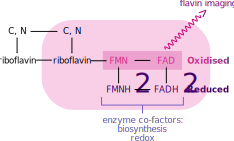
\includegraphics[width=0.8\textwidth]{flavin-cell-schematic}
  \caption[
    Simplified schematic of biosynthesis of flavins
  ]{
    Simplified schematic of biosynthesis of flavins and detection of the oxidation states in fluorescence microscopy.
    }
  \label{fig:intro-flavin-schematic}
\end{figure}

Riboflavin can be synthesised \textit{de novo} from purine biosynthesis and the oxidative pentose phosphate pathway (Fig.\ \ref{fig:intro-flavin-kegg}).
% Is there more to this than the KEGG diagram?
Based on the metabolism of flavins, the cell only synthesises new flavin for synthesis of FMN and FAD\@; therefore, monitoring of flavins monitors the combined pool of FMN and FAD in their oxidised states.

% https://www.genome.jp/pathway/map00740
\begin{figure}
  \centering
  \includegraphics[width=1.0\textwidth]{kegg-flavin}
  \caption[
    Reference pathway for biosynthesis of riboflavin and derivatives
  ]{
    Reference pathway for biosynthesis of riboflavin and derivatives, KEGG pathway database \parencite{kanehisaKEGGTaxonomybasedAnalysis2023}.
    }
  \label{fig:intro-flavin-kegg}
\end{figure}

From a technical standpoint, the redox states of flavins reflect the emission and absorption of electromagnetic radiation by the flavin moiety.
The redox biochemistry of flavins give rise to fluorescence, so monitoring flavin autofluorescence monitors the redox state of the cell.
Flavins, in their oxidised forms (FMN and FAD), have a peak excitation frequency of $\approx$460 nm and a peak emission frequency of $\approx$535 nm \parencite{maslankaAutofluorescenceYeastSaccharomyces2018, wagnieresVivoFluorescenceSpectroscopy1998}, displayed in Fig.\ \ref{fig:intro-flavin-spectra}.
Comparison of \textit{in vivo} autofluorescence in mammalian cells and the fluorescence spectrum of riboflavin in PBS confirms this fluorescence behaviour \parencite{aubinAutofluorescenceViableCultured1979}.
In contrast, the reduced forms FMNH\textsubscript{2} and FADH\textsubscript{2} have negligible fluorescence \parencite{mastersConfocalRedoxImaging1994}.
Both chemostat-based \parencite{sasidharanTimeStructureYeastMetabolism2012, murrayRedoxRegulationRespiring2011} and single-cell microfluidic studies \parencite{baumgartnerFlavinbasedMetabolicCycles2018} have monitored flavin autofluorescence to study the YMC\@.

\begin{figure}
  \centering
  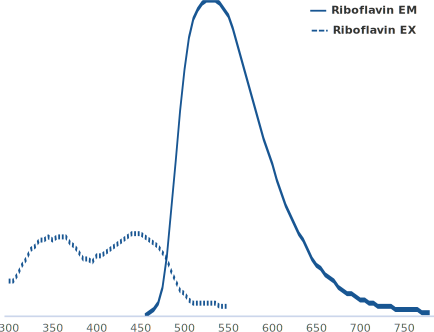
\includegraphics[width=0.9\textwidth]{fpbase-riboflavin-adapted}
  \caption[
    Fluorescence spectrum of riboflavin
  ]{
    Fluorescence spectrum of riboflavin, (dotted line) excitation and (solid line) emission spectra shown, FPbase \parencite{lambertUsingFPbaseFluorescent2023}.
    }
  \label{fig:intro-flavin-spectra}
\end{figure}

\subsubsection{Descriptions of key flavoproteins and their roles}
\label{subsubsec:intro-flavin-biochem-descriptions}

\textcite{gudipatiFlavoproteomeYeastSaccharomyces2014} describe 68 genes that code for 47 flavoproteins in budding yeast (Fig.\ \ref{fig:intro-flavoprotein-abundance}).
Of these, 35 require FAD, 15 require FMN, and 3 require both.
In budding yeast, most flavins sit in the active site without covalent bonding.
The biochemical and enzymatic properties of many flavoproteins are poorly characterised \parencite{kochStructureBiochemicalKinetic2017}.

\begin{figure}
  \centering
  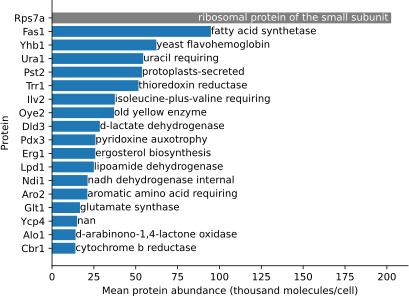
\includegraphics[width=0.9\textwidth]{flavoprotein_abundance_bar}
  \caption[
    Flavoproteins shown by abundance
  ]{
    Flavoproteins (blue bars) shown by abundance \parencite{hoUnificationProteinAbundance2018}, with Rps7ap (grey bar) shown as reference.
    Only the 17 most abundant flavoproteins are shown.
    }
  \label{fig:intro-flavoprotein-abundance}
\end{figure}

The most abundant flavoproteins catalyse redox reactions (Table~\ref{tab:intro-flavoproteins}).
Specifically, these reactions include reduction of reactive chemical species to respond to oxidative stress --- though not all enzymes involved in the response to reactive chemical species have flavin co-factors.
Additionally, the reactions include biosynthetic reactions.
Many of these reactions require NADPH or NADH to donate electrons, suggesting a link between flavins and NAD(P)H in regulating the cellular redox state.
In particular, Oye2p catalyses the NADPH redox reaction, thus providing a link between flavins and NAD(P)H\@.
One exception flavoprotein is Ilv2p, which does not catalyse a redox reaction.
It has been hypothesised that an ancestral form of Ilv2p catalysed a redox reaction, but the argument is weak because it is inferred from the presence of FAD \parencite{pangCrystalStructureYeast2002}.
To maintain the cellular redox state, it is thus reasonable to assume that the redox equilibrium of all flavoprotein-catalysed reactions are in the same direction at any point of the YMC\@.
Supporting this, \textcite{sianoNADHFlavinFluorescence1989} show that NAD(P)H fluorescence and the fluorescence of lipoamide dehydrogenase, a flavoprotein, indicate simultaneous reduction in response to lowered dissolved oxygen.
They further show redox equilibrium in both fluorophores in response to glucose addition.

\begin{table}[htbp]
  \footnotesize
  \centering
  % Control spacing between rows
  \renewcommand{\arraystretch}{2}
  \begin{tabularx}{\linewidth}{sbbs}
    \toprule
    Protein & Name & Reaction catalysed & Reference\\
    \midrule
    Fas1 & beta subunit of fatty acid synthetase & \ce{acetyl-CoA + malonyl-CoA + NADPH + ATP -> palmitate} & \textcite{singhDiscoveryRegulatorySubunit2020} \\
    Yhb1 & nitric oxide oxidoreductase & \ce{2NO + 2O2 + NAD(P)H -> 2NO3- + NAD(P)+ + H+} & \textcite{bonamoreFlavohemoglobinStructureReactivity2008} \\
    Ura1 & dihydroorotate dehydrogenase & \ce{dihydroorotic acid + fumarate -> orotic acid + succinate} & \textcite{zameitatDihydroorotateDehydrogenaseSaccharomyces2007} \\
    Pst2 & NAD(P)H-quinone oxidoreductase & \ce{NAD(P)H + H+ + quinone -> NAD(P)+ + hydroquinone} & \textcite{kochStructureBiochemicalKinetic2017} \\
    Trr1 & cytoplasmic thioredoxin reductase & \ce{H+ + NADPH + thioredoxin disulfide -> NADP+ + thioredoxin} & \textcite{machadoThioredoxinReductasedependentInhibition1997} \\
    Ilv2 & acetolactate synthase & \ce{2 pyruvate -> 2-acetolactate + CO2} & \textcite{pangCrystalStructureYeast2002} \\
    Oye2 & NADPH oxidoreductase & \ce{NADPH + H+ + acceptor <--> NADP+ + reduced acceptor} & \textcite{odatOldYellowEnzymes2007} \\
    Dld3 & 2-hydroxyglutarate transhydrogenase & \ce{D-2-hydroxyglutarate + pyruvate -> \alpha-ketoglutarate + lactate} & \textcite{becker-ketternSaccharomycesCerevisiaeForms2016} \\
    Pdx3 & pyridoxine phosphate oxidase & \ce{pyridoxamine 5-phosphate + H2O + O2 -> pyridoxal 5-phosphate + NH3 + H2O} & \textcite{tsugePurificationPropertiesPyridoxamine1979} \\
    Erg1 & squalene epoxidase & \ce{squalene + H+ + NADPH + O2 -> 2,3-oxidosqualene + NADP+ + H2O} & \textcite{satohEnzymaticPropertiesSqualene1993} \\
    Lpd1 & dihydrolipoamide dehydrogenase & \ce{dihydrolipoamide + NAD+ -> lipoamide + NADH+ + H+} & \textcite{morrisonChapter14Dihydrolipoamide2021} \\
    \bottomrule \\
  \end{tabularx}
  \caption{
    Roles of the most abundant flavoproteins.
  }
  \label{tab:intro-flavoproteins}
\end{table}

It is important to rule out the possibility that flavin cycling is merely a function of the cell division cycle to make sure that flavin monitoring monitors the YMC\@.
None of these flavoproteins are strictly cell division cycle proteins, but this does not exclude cycling of flavin autofluorescence linked to the cell division cycle.
For example, fatty acid synthesis proteins should cycle along with the cell division cycle as cell synthesises more plasma membranes.

\subsection{Flavins and flavoproteins in the yeast metabolic cycle}
\label{subsec:intro-flavin-ymc}

Flavin fluorescence can be used to monitor the metabolic cycle.
The biological basis of flavins justifies this use.
Flavins are linked to NAD(P)H via nitric oxide oxidoreductase (Yhb1p), as discussed in Section~\ref{subsubsec:intro-flavin-biochem-descriptions}, and NAD(P)H cycles have been implicated in bulk-culture \parencite{tuLogicYeastMetabolic2005} % and more
and single-cell \parencite{papagiannakisAutonomousMetabolicOscillations2017} studies of the YMC, as discussed in Section~\ref{subsubsec:intro-ymc-definition-phases}.
The oxidation of flavin is at its maximum at the start of the reductive state of the YMC, as evidenced by how flavin fluorescence peaks just before dissolved oxygen concentration in the chemostat \parencite{murrayRedoxRegulationRespiring2011,sasidharanTimeStructureYeastMetabolism2012}.
Riboflavin abundance in the cell has been shown to oscillate and peak in the oxidative state of the YMC, while FAD abundance is at its maximum in the reductive-building phase, as evidenced by metabolic profiling of extracts from chemostat cultures taken at evenly-spaced intervals \parencite{tuCyclicChangesMetabolic2007}.

Flavoproteins may have roles linked to the YMC\@.
The most abundant is Fas1 (fatty acid synthetase).
Because there is evidence that cycles of fatty acid stores are implicated in metabolic cycling in yeast \parencite{campbellBuildingBlocksAre2020}, it is likely that fatty acid synthetase is heavily implicated.
Following this, the second most abundant is Yhb1, which may play a major role as discussed earlier.

So, for these reasons, I expect flavin autofluorescence to be oscillatory and be a useful readout of the yeast metabolic cycle.
Few studies have characterised how such flavin oscillations respond to changing nutrient conditions or to gene deletions.
Thus, filling in this knowledge gap is an avenue for further research.

Nevertheless, there are caveats to using flavin autofluorescence.
Riboflavin fluorescence is captured too, though its intracellular abundance is two order of magnitudes lower than that of FMN and that of FAD, and these two flavin derivatives are present at the same order of magnitude \parencite{tuCyclicChangesMetabolic2007}.
In addition, different concentrations of riboflavin influence the autofluorescence signal and influence the physiological state of the cell \parencite{maslankaAutofluorescenceYeastSaccharomyces2018}.
However, the experimenter can eliminate the effects of riboflavin by using riboflavin-free minimal media \parencite{verduynEffectBenzoicAcid1992}.
Additionally, flavin fluorescence is the aggregate of many flavoprotein components, therefore it cannot be concluded that flavin fluorescence is the readout of one protein in particular --- one can only draw conclusions about the overall redox state.
Furthermore, the changes in flavin fluorescence can be because of changes in the `flavin pool' --- the amount of flavin-derived moieties in a cell across all their redox states --- or due to global changes in intracellular flavin redox state, as a function of intracellular redox state.
Most studies assume a constant flavin pool and see oscillations as periodic shifts in redox equilibrium.
These caveats are not unique to flavin fluorescence, but are shared limitations with other auto-fluorescing cellular components like NAD(P)H, and the benefits of having a non-invasive method to monitor cellular metabolism outweighs the caveats.

%%% Local Variables:
%%% mode: latex
%%% TeX-master: "../thesis.tex"
%%% End:
